\documentclass[12pt,a4paper]{article}
\usepackage{setspace}
\usepackage[top = 1.25in, bottom = 1.25in, left = 1.25in, right = 1.25in]{geometry}
\usepackage[utf8]{inputenc}
\usepackage{amsmath}
\usepackage{amsfonts}
\usepackage{amssymb}
\usepackage{amsthm}
\usepackage{graphicx}
\usepackage{natbib}
\usepackage{caption}
\usepackage{subcaption}
\usepackage{float}
\usepackage{pdflscape}
\usepackage{booktabs}
\usepackage{dcolumn}
\usepackage{pdflscape}
\usepackage[hyphens]{url}
\usepackage{enumitem}
\usepackage[table]{xcolor}
\usepackage{authblk}
\usepackage{appendix}
\usepackage{titletoc}
\setlength\parindent{20pt}
\usepackage{setspace}
\usepackage{multirow}
\usepackage{caption}
\usepackage{titling}
\usepackage{amsmath}
\DeclareMathOperator*{\argmax}{arg\,max}
\onehalfspacing
\usepackage[hang,flushmargin]{footmisc}

\newtheorem{theorem}{Theorem}[section]
\newtheorem{lemma}[theorem]{Lemma}
\newtheorem{proposition}{Proposition}
\newtheorem{corollary}{Corollary}
\renewcommand{\theproposition}{\arabic{proposition}}
\newcommand{\real}{\mathbb{R}_+^n}
\newcommand{\bfv}{\mathbf{v}}
\newcommand{\blue}{\textcolor{blue}}

\bibliographystyle{unsrtnat}
\begin{document}

\section{Introduction}

Across the world, vulnerable populations rely on governments for access to basic public services such as education. Over the past two decades, enrollment rates in public education have improved dramatically.\footnote{See \citet{haggard_development_2008}, \citet{kaufman_globalization_2001}.} Improvements in access have not been matched, for many, with a better quality of education. From a global perspective, educational quality indicators such as the PISA (Programme for International Student Assessment) score have broadly stagnated.\footnote{For coverage, see [here](https://www.economist.com/international/2019/12/05/pisa-results-can-lead-policymakers-astray).}

How can we improve the quality of education? In large part, the answers are domestic. While each country faces a particular set of challenges, broad institutional reforms in the developing world make their cases comparable. Decentralization has delegated responsibility for public education to subnational governments, as well as induced variation in the quality of education along subnational lines \citep{falleti_decentralization_2010, arretche_mitos_1996}. Understanding how this level of government manages these services, and in particular how local actors strategically shape them can help find answers to that question. \citep{gulzar_politicians_2017, min_power_2015}.

% In this paper, I highlight the role of the strategic interaction between political elites and its downstream effects on the provision of educational services. Similar to coalition building, local executive leaders secure broader support for their policy agenda through the allocation of public sector positions to city councilors.^[@laver_coalitions_1990, @power_optimism_2010.] As highlighted by previous research, teacher turnover can lead to decreased morale and inexperienced staff entering public service (@ingersoll_teacher_2001, @ronfeldt_how_2013). Patronage, by inducing new hires or dismissals, can therefore cause instability in the educational sector, with negative effects for student learning.

% To estimate the effect of patronage on quality of education, I combine qualitative and quantitative evidence. Interviews conducted with educational bureaucrats and politicians confirm that turnover has a negative impact on teachers' ability to educate students. To validate these accounts I combine administrative data on education, both at a national and subnational level. I construct a multiple datasets to test these claims: the main specification contains over 1 million classrooms spread across the national territory, and a school-grade-specific turnover index. A set of estimations, combining multi-level modeling and fixed effects, provide strong evidence that teacher turnover has a negative effect on student learning.

% To analyze how politics affect staff turnover, I analyze the relationship between municipal education staff turnover and the share of seats controlled by the executive in the local city council. In line with qualitative accounts and theoretical expectations, mayors who face stronger legislative opposition resort to greater patronage, in particular during the first year of administration. Mayors therefore resort to patronage in order to shore up legislative support, with negative consequences for student learning. I leverage data on over 2 million school teachers and school principals to estimate the effect of share of executive seats on turnover. Different model specifications confirm that turnover increases (decreases) as the share of seats held by the mayor coalition decrease (increase).

% This study contributes to an emerging literature on the politics of personnel and public services (@pepinsky_bureaucracy_2017, @finan_personnel_2015 and @gulzar_politicians_2017). Focusing on political actors refines our understanding of local politics and how intra-elite bargain reshape bureaucracies, leading to welfare loss for the broader population, as subnational actors divert resources from public services (@ferraz_corrupting_2012). It also shifts focus from provision to the implementation of public services, echoing a long-standing literature on state capacity and the necessity for bureaucratic autonomy (@kohli_state-directed_2004, @evans_embedded_1995).

% The paper is structured as follows. Section 1 provides an overview of the scholarly debate over public goods provision and personnel, as well as more specific treatments of the subject in Brazil. In section 2 I present the main theoretical argument, with a formal treatment of the subject. Section 3 presents the institutional context and data, followed in section 4 by the research design and main results. Section 5 concludes.

% # Related literature and debate

% In this section I review extant literature on public goods provision and the politics underlying it, focusing on more recent studies of bureaucratic personnel and political leaders reshape these institutions. I also highlight how my research incorporates multiplicity in political actors and how this affects bargaining over public sector jobs. I address this gap by adapting previous analyses of executive-legislative bargaining to bureaucratic control at the local level.

% ## Bureaucratic personnel and public goods provision

% Bureaucracies have a clear impact on the delivery of public services. A long-standing literature on state capacity provides a theoretical and substantive foundation to analyze bureaucratic institutions (@centeno_unpacking_2017, @kohli_state-directed_2004). A first generation of scholars, focusing on the successful developmental cases of East Asia, highlighted the need for a technocratic and autonomous bureaucracy (@johnson_miti_1982, kohli_state-directed_2004). A Weberian wall separating bureaucrats from elected officials was considered indispensable for the successful provision of economic growth (@evans_bureaucracy_1999).

% Recent studies have added nuance to these claims, finding that high bureaucratic performance can coexist with political interference. Toral 2019 finds in Brazil that school principals appointed by mayors tend to perform better than their non-appointed counterparts in standardized test scores. @gulzar_politicians_2017 show that local politicians who are able to internalize electoral benefits make bureaucrats exert more effort, increasing local employment. @akhtari_political_2015, on the other hand, highligh the pitfalls of political capture, showing that party turnover can lead to the replacement of school principals, with detrimental effects for student learning.

% This recent wave of studies shed light on the intersection between politicians and bureaucracies. However, few of these studies explicitly model the multiple actors involved in managing bureaucracies. Understanding their diverse goals and action space provides a firm theoretical foundation to how different politicians can reshape bureaucracies. To do so I turn to the well-established literature on executive-legislative bargaining, applying its insights to the analysis of local government and administration.

% ## Presidential coalitionism and patronage

% For every elected mayor in Brazil, a group of legislators are also elected into office. These political actors have competing claims over the local bureaucracy, with important implications for public service delivery. This structure parallels other settings with an institutinalized separation of powers and a bureaucratic pie to be split among the actors (@grindle_jobs_2012, @mccarty_appointments_2004). Divergent political interests can lead to strategic interaction between executive and legislative actors. A rich literature in Brazil explores these relations, with important insights to how executive and legislators bargain over bureaucracy. (@raile_executive_2011, @power_optimism_2010). 

% In the Brazilian federal context, executive-legislative relations are analyzed under the prism of presidential coalitionism. Executive leaders garner legislative support from the National Congress by exchanging key positions in the federal bureaucracy, appointing members of their legislative coalition into cabinet positions. (@raile_executive_2011). In a setting characterized by weak party cohesion and programmatic commitments (@ames_electoral_1995, @lucas_ideological_2010), bureaucratic positions for members of the coalition provide material incentives for legislators to support the executive agenda (@batista_o_2013, @neto_presidential_2006, @figueiredo_executivo_1999).

% \blue{something about coalitions}

% In municipalities, mayors have to garner legislative support from city councilors to secure budgetary approval and implement desired policies. Due to weak programmatic commitments at the local level, public sector jobs are used to legislative support.^[Interview with C, August and September 2019.] Mayors enjoy full discretion into how to appoint workers into the public sector, and use patronage to coopt legislative support from members of the coalition, a practice known locally as \textit{empreguismo}. As noted by a former mayor of the municipality of Sobral, "city councilors knocked on my door with a list of names for people they wanted me to hire."^[Interview with C, August 2019.] These hires induce changes in personnel, with important consequences for bureaucracies and educational services.

% ## Bureaucratic turnover and inexperienced education

% Bureaucracies exposed to turnover experience productivity shocks, often with detrimental effects. As new staff enters the bureaucracy, they must learn and acquire skills to deliver services to the population (@gailmard_slackers_2007). Focusing on education, studies show that students taught by inexperienced teachers perform worse than those attending class with an experienced teacher (@clotfelter_teacher_2007.) @akhtari_political_2015 finds that students attending a school with a recently appointed school principal perform worse in standardized test scores. When bureaucratic turnover is driven by patronage, political concerns take precedence over meritocratic ones (@colonnelli_patronage_2017).

% > "I am aware that the position is temporary. Especially because it is a political position, decided by the administration. If the current administration is out of power, we are automatically dismissed." - Interview with school principal A, August 2019.

% Negotiations between executive and the legislative thus have a knock-on effect on the quality of educational services, as political considerations lead to bureaucratic turnover at the school and administrative level. In this study, the primary focus is on bureaucrats working within the boundaries of a school: school principals and teachers. In the following section I describe the institutional context for public education in Brazil, as well as the data employed for the the estimation.

% # The argument

% ## The executive dilemma

% I model the executive decision over patronage as a product of political career concerns and strategic interaction with the local legislative power. In particular, mayors are assumed to be career-oriented and re-election seeking (@besley_principled_2006). This provides an alternative set-up to extant treatments of patronage as a pre-electoral bargain, naturally highlighting the question of government performance (@stokes_brokers_2013, @robinson_political_2013.) The key feature of the model is the trade-off between patronage and quality of public services, which mayors are aware of when allocating public sector jobs to city councilors.

% The mayor's strategy centers around the redistribution public sector jobs. When the mayor takes office, a set of bureaucratic positions become available for allocation to city councilors. In a municipal parallel to presidential coalitionism, jobs are allocated to legislators in order to buy their vote. I assume, for now, that job allocations have a negative effect on public services. The mayor can refrain from distributing jobs for vote buying, since reducing turnover helps retain expertise and improves the quality of public services. However, doing so raises the threat of defection by coalition members, which can lead to the withholding of budgetary approval. This is the executive's dilemma.

% The main proposition is that mayors who control a smaller (larger) share of legislative seats allocate more (less) public sector job to city councilors. The intuition is as follows. Mayors need to secure a simple majority of legislative votes to have the budget approved. @groseclose_buying_1996 and @banks_buying_2000 point out that the executive should prioritize votes from cheaper legislators, which in this set-up are those who share the same electoral coalition as the mayor. Having exhausted these votes, the executive has to resort to buying votes from the opposition, which demand more patronage. The less seats occupied by members of the mayor's electoral coalition, the more expensive vote-buying becomes, and the observable implication is increased patronage in the municipality.

% The model builds on rich theoretical treatment of electoral accountability and majority-buying in legislatures. Starting with @barro_control_1973 and @ferejohn_incumbent_1986, political economists have proposed formal models analyzing the nexus of electoral accountability as an incentive for shaping the behavior of elected politicians (@coate_form_1995; @besley_principled_2006). The possibility of reelection can motivate them to exert effort and convince voters to reelect them. This model extends previous analyses by incorporating legislators to the game, with the need to secure a legislative majority to implement the executive agenda (@groseclose_buying_1996, @banks_buying_2000).

% ## The model

% There is one mayor $m$, a city council $N$ and representative median voter $v$. The goal of the mayor is to be reelected into office, yet for any given time period $m$ needs to garner legislative support. The city council plays that key role by approving or not the budget for the executive. The legislative chamber is composed by $N = {1,..,n}$ legislators, where $S \subseteq N$ denote the subset of legislators who belong to the electoral coalition of mayor $m$. For each $i \in N$, let $\textbf{v} = \{v_1,...,v_n\}$ describe legislator i's preference to support the mayor in the budgetary process. Let $v_i > v_j$ for all $i \in S$ and $j \in \{N \setminus S\}$. Therefore, members of the mayor's electoral coalition are more likely to approve the budget than outside members.

% I introduce a set of simplifying assumptions. First, mayors are one of two types: a technocratic politician who delivers high quality public goods, and a pragmatic one, who fails to do so. Note that this is an informational heuristic. Voters have beliefs about how competent a politician is and strictly prefer them over the alternative. Because voters cannot observe the type, they update beliefs observing the quality of public goods they observe (@coate_form_1995). Additionally, I assume that the voter is sincere, excluding pivotality concerns and strategic voting from voters' utility calculations. Finally, I normalize the politician's exit option to 0: the politician always prefers to be re-elected.
 
% The game has two periods. Voter $v$ does not observe the amount of patronage handed out by mayor $m$ nor her type, but observes and derives utility from the realization of public good quality $\omega_t$. An important feature in the model is that high quality public services $\omega_{h}$ are produced probabilistically as a function of $\theta$, the quality of the bureaucracy. The more jobs a mayor allocates to legislators, the lower is $\theta$, thus capturing the inverse relation between patronage and state capacity.^[See @kohli_state-directed_2004.] The budgetary process also affects the public service delivery, with a failure to approve the budget lowering the resources available to the executive.

% The mayor's optimal strategy is pinned down by the share of patronage which maximizes expected utility from holding onto office, conditional on her type and expected benefits from reelection. Mayor $m$ has to offer public sector jobs to coopt the opposition while ensuring that the voter is satisfied enough to reelect her. The executive dilemma is how to reconcile the incentive for reelection and the pressure imposed by the opposition.

% The timing of the game is as follows.

% 1) Nature draws the politician's type.
% 2) Politician observes her type and allocates public sector jobs to legislators, setting $\theta_1$.
% 4) Nature realizes public good $\omega_1(\theta_1)$.
% 5) Voter observes $\omega_1$ and casts vote to retain or fire the incumbent.
% 6) If incumbent is retained, she sets $\theta_2$ and nature draws $\omega_2(\theta_2)$. If incumbent is deposed, a challenger takes office, sets $\theta_2$ and the game ends.

% ## The executive dilemma

% The mayor's choice set is the bureaucratic quality parameter $\theta_t$. As quality increases - the mayor allocates a smaller proportion of jobs to legislators - the less votes become secure in the legislature. This reduces the likelihood of securing the necessary resources to provide public goods for a given fiscal year. Adapting @gailmard_slackers_2007, there are two types of mayors: technocratic and pragmatic. Technocratic politicians invariably deliver high quality public goods to the voter. Pragmatic politicians, on the other hand, are susceptible to legislative pressure and at times fail to deliver them.

% The probability of a politician being technocratic is common knowledge: $\xi \in [0,1]$. Conversely, the probability of her being pragmatic is simply $1 - \xi$. Both types derive utility from public goods provision $\omega$, where for simplicity $u(\omega_l)=0$ and $u(\omega_h) = 1$. We do not model the decision of the competent mayor: she simply delivers high quality goods and is inevitably reelected. We focus on the more interesting case of the pragmatic mayor.

% \begin{align*}
% Eu_m \left(\theta_t, s_1 \middle|\lambda \right) &= \textbf{E}(\omega_1) + \delta \text{Pr}(\text{reelection})\left[\psi + \textbf{E}(\omega_2)  \right] \\
% &= \frac{1-s_1\theta_1}{1+e^{-(10\theta_1-5)}} + \delta \text{Pr}(\text{reelection})\left[\psi + \frac{1-s_2\theta_2}{1+e^{-(10\theta_2-5)}} \right] \\
% \end{align*}

% The equation above formalizes the mayor's dilemma. The probability of reelection decreases with the share of jobs allocated to the opposition, since it lowers the quality of the bureaucracy. However, if the mayor fails to appease them through patronage, it is increasingly costly to "govern". While technocrats are immune to these political pressures, pragmatists ultimately cave in. The need to coopt legislators decreases the quality of the bureaucracy and public goods, as mayors are forced to allocate positions within the bureaucracy to garner support in the legislative. Details on deriving the equilibrium strategy are in the appendix. I now describe Brazil as a case for testing the theory.

% # Institutional context and data

% ## Education in Brazil

% In Brazil, responsibility for primary education is delegated to local governments (@paschoal_historia_2009). The municipal educational system has increased in relevance over the past few decades, as municipalities took on a larger proportion of students from state-level governments. Figure \ref{fig:enrollment} plots the total number of students in primary education per government level, including private schools. As of 2016, over 25 million students were enrolled in over 115 thousand municipal schools.

% \blue{plots/enrollment_dep.pdf}

% The local executive branch has sole prerogative over the hiring and firing of teachers and school principals. School principals are considered positions of trust (\textit{cargos de confiança}) and usually appointed by the mayor or secretary of education (@brollo_political_2017). Teachers usually enter the public service through a public exam and are eligible for tenure after two years (@gatti_formacao_2010) However municipalities increasingly resort to temporary contracts to hire new teachers as budgetary pressures amount. Municipal teachers and school principals are overseen by a local department of education (@militao_educacao_2014).

% Funding for municipal education relies primarily on federal transfers, the Fundeb, derived from 10 percent of tax revenues for each level of government to education. At the municipal level, 25 percent of the local budget must be allocated to education, and compensatory federal transfers are institutionalized by law to those municipalities which do not reach the target.^[For more details on the Fundeb, see (here)[https://www.fnde.gov.br/index.php/financiamento/fundeb/sobre-o-plano-ou-programa/sobre-o-fundeb].] While municipalities may be audited to verify whether funds are being properly used, personnel decisions and daily operations are fully under municipal discretion (@ferraz_corrupting_2012).

% ## Local governance and mayoral coalitions

% Brazil is comprised by over 5 thousand municipalities, each with their own city hall and council. Mayors and city councillors (\textit{vereadores}) are democratically elected every four years, with the possibility of reelection for both.^[The last municipal elections were in 2016. These take place ] The executive is responsible for the implementation of social policies such as education, as well as drafting the municipal budget. The city council, on the other hand, oversees legislation and approves the budget for the fiscal year. As noted by @souza_reforma_2004, decisions over how to manage education are primarily in the hands of the mayor, but the city councilors exert significant pressure.

% In order to win elections and garner support for their campaign, mayors form electoral alliances with local party labels (@dantas_eleicoes_2013). These mayoral coalitions, once in government, are an important basis for approving budgets and, more generally, executive control over the legislative chamber. Interviews with city councilors indicate that the legislature is divided into a pro-government (\textit{governo}) and opposition (\textit{oposição}) groups (\textit{bancada}). While these electoral coalitions do not necessarily remain intact once governments are formed, fragmentation is generally on the margins, with mayors swapping defecting legislators for new ones.^[Interview with C, former chief of staff of municipality J. September 2018.]

% Interviews with secretaries of education and mayors suggest that city councilors play an important role in staffing decisions. While mayors hold jurisdiction over personnel decisions, there are extensive consultations between mayors and city councilors to decide who becomes the principal of a school, or which teacher remains in a school or leaves. These executive-legislative consultations ultimately determine the allocation (\textit{alotação}) of educational staff, serving as the primary tool through which mayors reward or coopt legislators into supporting them in the city council. In the words of a set of school administrators in the municipality of I:

% > School principal: Here, we are invited to work at the school by the department of education, with the [political] candidate, the city councilor...deciding which are the positions they are searching for and appointing people they think have the necessary qualifications.

% > Educational counselor: I was also invited to work here, by the city councilor and the department of education.^[Interview with the administrative board of school A., municipality J. August 2019]

% These accounts, along with previous case studies of municipalities in Brazil, suggest that city councilors play an important role in nominating staff. To verify these claims in a broader set of municipalities, as well as outlining the research design, I employ extensive administrative and electoral data collected by the Brazilian federal government. In the next section I describe the data, where it is publicly available, as well as the preparation necessary for the set of estimations presented in the study.

% ## Data

% Brazil collects fine-grained data on education and makes it publicly available for research. For this study, data on education are collected from two main sources: the SAEB and School Census.^[These can be accessed (here)[http://portal.inep.gov.br/web/guest/dados].] The SAEB (National System for Educational Assessment) is a biannual standardized exam administered by the INEP (National Institute fosr Educational Studies and Research) to all public schools and a sample of private schools. In 2017, over 5 million students, in 5th and 9th grade, took the exam, testing their proficiency in both mathematics and Portuguese. In this study, test scores are the primary metric for assessing the quality of education received by students.

% \blue{"plots/saeb_map.pdf"}

% Figure \ref{fig:map} presents a map of Brazil with the municipal averages for the SAEB of 2015. Warmer colors such as red and orange indicate higher average scores, with the converse denoted by colder, blue shades. There is clear variation in average test scores, with the Southeast and Midwest outperforming poorer regions in the North and Northeast. Even within regions, however, there is wide heterogeneity. In particular, note that in the northern part of Brazil, high-performing municipalities neighbor low-performing ones. This indicates that despite spatial clustering, municipal factors can lead to variation in the quality of education.

% Employment data on educational staff, including teachers and school principals, are extracted from the RAIS, SAEB and the School Census.^[RAIS data, along with additional Brazilian employment data, can be accessed (here)[http://trabalho.gov.br/dados-abertos].] The \emph{Relatório Anual de Informações Sociais} (RAIS) is an annual census administered by the now Ministry of Finance to all formal employers in Brazil. Employers are mandated to accurately report data on employees, subject to fines for misreporting. Subnational governments, including municipalities, also report to the RAIS. The dataset therefore contains micro-level information on all municipal personnel, including when they were hired/fired, as well as wages, type of contract and education levels.

% Figure \ref{fig:staff} provides descriptive statistics on bureaucratic personnel in Brazil, segmented by department. Educational staff, in this case school principals and teachers, comprise approximately a third of municipal public sector jobs, totaling around 2 million in 2015. While comparable to administrative staff, this total significantly exceeds that for healthcare services. Focusing on turnover, we note that new hiring and dismissals in education staff is relatively high. While lower than that for administrative staff, new hires can represent over 10 percent of extant staff. The past two decades was a moment of rapid expansion of municipal staff, and hiring has far exceeded dismissals in that time period.

% \blue{plots/turnover_category.pdf}

% I propose three different specifications for measuring bureaucratic turnover. From the RAIS I obtain the percentage of teachers and principals who are dismissed and hired at any given year. Using school census data, it is possible to track individual teachers across time and schools. With that data I calculate a turnover index for school $s$, in municipality $j$ at year $t$, based on an index proposed by @pereira_junior_indicadores_2016. The number of teachers leaving and entering the school at a given year are summed and divided by the total number of teachers in the current and previous period.

% $$\text{turnover}_{sjt} = \frac{\text{exit}_{sjt} + \text{entry}_{sjt}}{N_{sjt} + N_{sjt-1}}$$

% Information on mayor, city councilors and mayoral coalitions are made available by the Supreme Electoral Court (TSE), the national authority responsible for overseeing elections.^[Available (here)[http://www.tse.jus.br/eleicoes/estatisticas/repositorio-de-dados-eleitorais-1].] In order to calculate the share of legislative seats held by the mayoral coalition, I match the partisanship of each city councilor to the mayoral electoral coalition. The distribution of share of coalition seats is depicted in figure \ref{fig:coalition}. Note that although most city councils are controlled by the mayor, in over 40 percent of municipalities the mayoral coalition is a minority government.

% \blue{plots of}

% Additional data has been collected to supplement the estimation exercise. Sociodemographic data comes from the National Institute for Statistics and Geography (IBGE), budgetary data from (FINBRA) and student test scores from Ceará (SPAEEC) are graciously provided by the Department of Education of Ceará.^[Respectively, data can be found here: (1)[https://ces.ibge.gov.br/base-de-dados/links-base-de-dados.html], (2)[https://siconfi.tesouro.gov.br/siconfi/pages/public/consulta_finbra/finbra_list.jsf], (3)[https://www.seduc.ce.gov.br/spaece/].]

% # Estimation

% ## Empirical strategy

% This study presents two sets of estimations. The first one identifies the effect of bureaucratic turnover on student learning, verifying the hypothesis that teacher and school principal turnover has a negative effect on the quality of municipal education. To do so, I leverage the test scores made available by SAEB and SPAECE to estimate the effect of turnover on student test scores. To avoid interference, individual test scores are aggregated at the classroom level, for each 5th and 9th grade of each school contained in the sample. The outcome of interest is thus the average test scores for all students in the same classroom (SAEB) or same grade (SPAECE), for a given school.

% For the first estimation, I employ a hierarchical linear model to estimate the effect of teacher turnover on average test scores for grade $i$ at school $s$, in municipality $j$ and year $t$. This estimation strategy has been used in multiple studies to analyze educational, due to its natural multi-level setting (classroom, school and municipality) as well as ability to incorporate covariates at each level of the estimation (@diprete_multilevel_1994, @lee_using_2000.) Let $\text{grade}_{isjt}$ be a dummy variable equal to 1 if the classroom is in grade 9 and 0 otherwise. The main specification is as follows:
% \begin{align*}
% \text{test score}_{isjt} = \beta_1 \text{turnover}_{isjt} + \beta_2 \text{grade}_{isjt} +\beta_3 \text{turnover}_{isjt} \times \text{grade}_{isjt} + \\ 
% \psi X_{isjt} + \phi V_{sjt} +\zeta W_{jt}+ \alpha_k + \delta_t + \epsilon_{isjt}
% \end{align*}
% We are interested in $\beta_1$ and $\beta_3$, the change in test scores associated with teacher or school principal turnover. In this set-up, $\beta_3$ is the additional effect of staff turnover on test scores if students are in 9th grade. The first level is the grade, with associated characteristics $X_isjt$ at the grade level: among others, percentage of students who have not graduated last year and share of children with a fridge in their house. The second is the school $s$, with characteristics $V_{sjt}$, such as access to internet or the presence of a cafeteria for students. The third level is the municipality $j$, including municipal sociodemographic characteristics ($W_{jt}$) such as population size and median wages, as well as per pupil budgetary expenditures on eduation. Finally, I include state ($\alpha_kj$) and year ($\delta_t$) fixed effects to account for unobserved time-invariant state characteristics and annual seasonality.

% The second set of estimations tests the hypothesis that mayors who control less seats in the city council engage in more patronage. To do so I leverage employment data from RAIS and school census data to measure teacher turnover rates. I deploy three sets of models. For the second and third estimation I turn to the micro, bureaucrat-level and a then to aggregated turnover at the municipal level. The first model is a logistic regression where the outcome of interest is whether a particular teacher or school principal is hired/fired for any given year. The second model is a linear model with fixed effects, where the outcome of interest is the proportion of educational staff hired/fired for a muncipality at any given year. For the second set of estimations, the main specification is:
% $$\text{turnover}_{jt} = \gamma \text{coalition seats}_{jst} + \mu P_{jt} + \zeta W_{jt}+ \alpha_k + \delta_t + \epsilon_{jt}$$
% The share of coalition seats held by the mayoral coalition is the treatment in this set-up. We are interested in $\gamma$, the change in bureaucratic turnover associated with variation in the share of legislative seats held by the mayoral coalition. Municipal characteristics $W_{jt}$ are similar to the ones used for the first set of estimation. I add political variables to the estimation in order to control for differences in mayor partisanship, incumbency status, and individual characteristics of the mayor: professional background, education, and age.

% Despite the use of different educational quality and staff turnover metrics, addition of a relatively extensive set of controls, the estimation strategy proposed here remains observational. In the absence of exogenous shock in either turnover or coalition shares, a credible identification strategy for each set of estimations remains a challenge. To partially address these concerns, as an additional robustness check I replicate these estimations with weights estimated through a covariate balancing propensity score outlined in @imai_covariate_2014 which is generalized for continuous treatments. A covariate balance test for either estimation is presented in the appendix.

% ## Results 

% Teacher and school principal turnover have significant, negative effects on average test scores, highlighting the potential dangers of bureaucratic turnover on student learning. These results are robust to alternative specifications of turnover, as well as the use of different quality metrics (SAEB, SPAECE) in our estimations. Table \ref{tbl:hlm_mods} presents the results of the estimation on SAEB test scores. We present two specifications for turnover. Turnover index measures the amount of turnover in teachers at the school level. Work experience for teachers and school principals serve as an alternative measure of turnover. Personnel who has only recently entered the school recently amass a shorter amount of work experience (less than two years).

% \begin{landscape}
% \begin{table}[t]
%   \centering
%   \footnotesize
%   
% Table created by stargazer v.5.2.2 by Marek Hlavac, Harvard University. E-mail: hlavac at fas.harvard.edu
% Date and time: Fri, May 22, 2020 - 02:22:04 PM
\begingroup 
\small 
\begin{tabular}{@{\extracolsep{5pt}}lcccc} 
\\[-1.8ex]\hline 
\hline \\[-1.8ex] 
 & \multicolumn{4}{c}{Student learning} \\ 
\cline{2-5} 
\\[-1.8ex] & \multicolumn{4}{c}{SAEB average test scores} \\ 
\\[-1.8ex] & (1) & (2) & (3) & (4)\\ 
\hline \\[-1.8ex] 
 Turnover index & $-$0.012$^{***}$ & $-$0.008$^{***}$ &  &  \\ 
  & (0.001) & (0.0004) &  &  \\ 
  Turnover index $\times$ Grade 9 & 0.002 &  &  &  \\ 
  & (0.001) &  &  &  \\ 
  Teacher experience (2 years) & $-$0.008$^{**}$ & $-$0.005$^{***}$ &  &  \\ 
  & (0.004) & (0.001) &  &  \\ 
  Teacher experience (10 years) & 0.007$^{**}$ &  &  &  \\ 
  & (0.003) &  &  &  \\ 
  School principal experience (2 years) &  &  & $-$0.033$^{***}$ & $-$0.009$^{***}$ \\ 
  &  &  & (0.0003) & (0.001) \\ 
  School principal experience (10 years) &  &  & $-$0.014$^{***}$ & $-$0.011$^{***}$ \\ 
  &  &  & (0.0003) & (0.0002) \\ 
  saeb\_teacher\_work\_schoolmore than 10 &  &  & $-$0.0005 & $-$0.002$^{***}$ \\ 
  &  &  & (0.0004) & (0.0004) \\ 
  saeb\_principal\_experience &  &  & $-$0.027$^{***}$ &  \\ 
  &  &  & (0.001) &  \\ 
  saeb\_principal\_experienceless than 2 years &  &  & $-$0.007$^{***}$ & $-$0.008$^{***}$ \\ 
  &  &  & (0.0002) & (0.0002) \\ 
  saeb\_principal\_experiencemore than 10 &  &  & 0.016$^{***}$ & 0.011$^{***}$ \\ 
  &  &  & (0.001) & (0.001) \\ 
 \hline \\[-1.8ex] 
Controls & \_ & \checkmark & \_ & \checkmark \\ 
Observations & 649,889 & 541,822 & 1,176,899 & 796,059 \\ 
\hline 
\hline \\[-1.8ex] 
\textit{Note:}  & \multicolumn{4}{r}{$^{*}$p$<$0.1; $^{**}$p$<$0.05; $^{***}$p$<$0.01} \\ 
\end{tabular} 
\endgroup 

%   \caption{{\bf Bureaucratic turnover and student learning} Teacher and school principal turnover have a negative effect on student learning. Models 1 and 2 present results for teacher turnover index constructed at the school level. Models 3 and 4 estimate the effect of new teachers and school principals entering the school (less than two years). All models include year and state fixed effects.}
%   \label{tbl:hlm_mods}
% \end{table}
% \end{landscape}

% Additionally, I present results for the SPAECE standardized exam in table \ref{tbl:spaece}. Differently than the SAEB, the SPAECE takes place annually and the average test scores are calculated at the grade, rather than the classroom level. The annual frequency of this exam allows us to retrieve more precise estiamtes with respect to the effect of teacher turnover on student test scores, as opposed to the biannual frequency of the SAEB. Note that for both estimations, we standardize the outcome of interest. Coefficients are therefore interpretable as a standard deviation change in student test with respect to the covariate.

% \begin{table}[t]
%   \centering
%   \footnotesize
%   
% Table created by stargazer v.5.2.2 by Marek Hlavac, Harvard University. E-mail: hlavac at fas.harvard.edu
% Date and time: Thu, Jun 11, 2020 - 04:05:22 PM
\begingroup 
\small 
\begin{tabular}{@{\extracolsep{5pt}}lcc} 
\\[-1.8ex]\hline 
\hline \\[-1.8ex] 
 & \multicolumn{2}{c}{Student learning} \\ 
\cline{2-3} 
\\[-1.8ex] & \multicolumn{2}{c}{SPAECE average test scores} \\ 
\\[-1.8ex] & (1) & (2)\\ 
\hline \\[-1.8ex] 
 Turnover index & $-$0.054$^{***}$ & $-$0.057$^{***}$ \\ 
  & (0.015) & (0.015) \\ 
  Turnover index $\times$ Grade 9 & 0.062$^{***}$ & 0.065$^{***}$ \\ 
  & (0.018) & (0.018) \\ 
 \hline \\[-1.8ex] 
Controls & \_ & \checkmark \\ 
Observations & 2,860 & 2,860 \\ 
R$^{2}$ & 0.552 & 0.556 \\ 
\hline 
\hline \\[-1.8ex] 
\textit{Note:}  & \multicolumn{2}{r}{$^{*}$p$<$0.1; $^{**}$p$<$0.05; $^{***}$p$<$0.01} \\ 
\end{tabular} 
\endgroup 

%   \caption{{\bf Turnover and student learning in Ceará.} Teacher turnover have a negative effect on student learning. Models 1 and 2 present results for teacher turnover index constructed at the school level.}
%   \label{tbl:spaece}
% \end{table}

% I now turn to testing the main proposition of this paper: that turnover in educational staff stems indeed from coalitional dynamics. There is strong evidence that mayors who control more (less) seats in the city council resort to less (more) patronage. Table \ref{tbl:turnover} presents the results of the estimation. The first model regresses turnover index on coalition share, where the unit of analysis is a grade-level per school. Models 2 and 3 estimate the effect of the share of legislative seats on hiring or dismissal of individual bureaucrats. The third set of models (4 and 5) estimate the change in the share of new hires and dismissals at the municipal level. All models suggest that an increase in the executive share of legislative seats decrease turnover.

% \begin{landscape}
% \begin{table}[t]
%   \centering
%   \footnotesize
%   
% Table created by stargazer v.5.2.2 by Marek Hlavac, Harvard University. E-mail: hlavac at fas.harvard.edu
% Date and time: Fri, Jul 03, 2020 - 12:37:34 PM
\begingroup 
\small 
\begin{tabular}{@{\extracolsep{5pt}}lcccccc} 
\\[-1.8ex]\hline 
\hline \\[-1.8ex] 
 & \multicolumn{6}{c}{Outcome} \\ 
\cline{2-7} 
 & \multicolumn{2}{c}{Turnover index (municipal)} & \multicolumn{2}{c}{Hires (municipal)} & \multicolumn{2}{c}{Hires (individual)} \\ 
\\[-1.8ex] & (1) & (2) & (3) & (4) & (5) & (6)\\ 
\hline \\[-1.8ex] 
 Share of legislative seats & $-$0.026$^{***}$ & $-$0.053$^{***}$ & $-$0.028$^{***}$ & $-$0.030$^{***}$ & $-$0.040$^{***}$ & $-$0.047$^{***}$ \\ 
  & (0.008) & (0.007) & (0.006) & (0.006) & (0.002) & (0.003) \\ 
  School principal &  &  & $-$0.252$^{***}$ & $-$0.245$^{***}$ & $-$0.222$^{***}$ & $-$0.386$^{***}$ \\ 
  &  &  & (0.015) & (0.017) & (0.013) & (0.015) \\ 
  Executive share of seats X School principal &  &  & $-$0.014 & $-$0.022$^{**}$ & $-$0.016 & $-$0.128$^{***}$ \\ 
  &  &  & (0.011) & (0.010) & (0.013) & (0.014) \\ 
 \hline \\[-1.8ex] 
Controls &  & \checkmark &  & \checkmark &  & \checkmark \\ 
State and year FE & \checkmarck & \checkmarck & \checkmarck & \checkmarck & \checkmarck & \checkmarck \\ 
Observations & 2,591,629 & 1,632,748 & 61,983 & 61,983 & 1,303,399 & 1,303,399 \\ 
R$^{2}$ & 0.027 & 0.045 & 0.184 & 0.296 &  &  \\ 
\hline 
\hline \\[-1.8ex] 
\textit{Note:}  & \multicolumn{6}{r}{$^{*}$p$<$0.1; $^{**}$p$<$0.05; $^{***}$p$<$0.01} \\ 
\end{tabular} 
\endgroup 

%   \caption{{\bf Executive coalitions and staff turnover.} An incrase in the share of legislative seats held by the mayoral coalition decrease the amount of turnover for teachers and school principals, including hires or dismissals. Model 1 presents results on the turnover index. Models 2 and 3 are logistic regressions at the individual, bureaucrat level. Models 4 and 5 are aggregated at the municipal level. where the outcome of interest is the proportion of staff either hired or dismissed at a given year. Models 1, 3, and 5 include year and state fixed effects.}
%   \label{tbl:turnover}
% \end{table}
% \end{landscape}

% For visual intuition, I present the predicted values for models 4 and 5, respectively the share of hired and dismissed bureaucrats against the share of executive seats in the city council. Albeit by construction the bivariate relationship is linear, it demonstrates that the amount of patronage is decreasing as executive coalition controls more seats in the legislature. Overall, these results suggest that weaker executive control over the legislature increases patronage, with potentially negative effects for public service delivery in municipalities in Brazil.

% \begin{figure}[H]
%     \centering
%     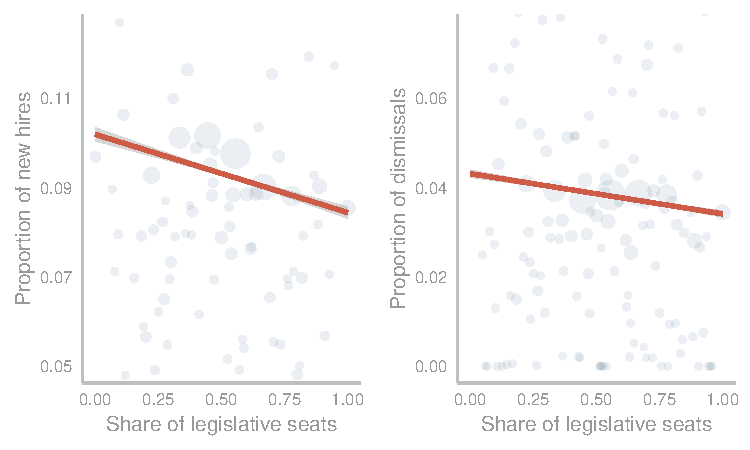
\includegraphics{plots/plot_pred}
%     \caption{Predicted values for bureaucratic turnover. The graph plots the proportion of educational staff either hired or fired for any given year against the share of seats controlled by the executive. The circles' size is proportional to the number of observations contained at each value of the legislative share of seats.}
%     \label{fig:turnover}
% \end{figure}

% As a final note, this set of estimations are based on observational data and therefore suffer from well-known concerns of endogeneity. It is in these circumstances that validating causal mechanisms through fieldwork and careful data analysis can increase the validity of a causal claim. In-depth interviews with local actors involved in managing education, as well as the use of different measurements for both educational staff turnover and student learning, provides strong evidence that staff turnover has a negative impact on student learning. Bureaucratic turnover stems from political considerations.

% ## Mechanisms

% The question remains: why do city councilors engage in patronage. Previous studies have found that citizens directly access 

% # Conclusion

% Improving the quality of education received by children across the world remains a challenge. This paper proposes an analytical framework and estimation strategy to understand the decision-making process behind the administration of educational services in Brazil. In a decentralized context, subnational political actors have a direct say on how educational services are managed, with profound implications for the quality of public services delivered to citizens. These actors interact with bureaucracies and other local elites in complex ways that are only beginning to be mapped.

% In this study I theorize and demonstrate that staff turnover stems from the executive's need to garner support from legislators in the city council. This process of coalition building is consolidated through employment offers to city councilors and their constituencies. As the share of seats held by the executive coalition decreases, the costlier it becomes to coopt legislators to support the executive. As a result, the amount of patronage we observe should increase. That is precisely what the data indicates, with teacher turnover increasing in schools, as well as increased hiring and dismissals of teachers and school principals.

% This bureaucratic turnover has important consequences for the quality of education delivered in municipalities. I find that turnover has a negative effect on student learning, across a set of specifications for turnover and different evaluation metrics for student learning. The evidence therefore seems to point out that mayors with a weaker hold on the city council resort to greater patronage, with negative consequences for student learning. This set of findings contribute to an emergent literature on the ambiguous consequences of stronger competition in weakly institutionalized contexts (@gottlieb_countervailing_2019).

% Future research on patronage and public service delivery would benefit from a clearer treatment of the institutional context in which local political actors operate. Important insights have been derived on executive leaders, but these actors seldom govern alone. Incorporating other local elites paints a more complex and accurate understanding of the strategic considerations taking place in the political management of education, and public services more broadly.

% \pagebreak 

% # Appendix

% \pagebreak

% ## Covariate balance

% ### Education quality vs. staff turnover

% \blue{plots/balance_hlm}

% ### Staff turnover vs. executive share of legislative seats

% \blue{plots/balance_felm.pdf}

% \pagebreak

\bibliography{dissertation}

\end{document}